\chapter{Modelos epidemiológicos en autómatas celulares}\label{ch:Modelos epidemiológicos en AC}

Podemos pensar en que si un individuo susceptible a una enfermedad tiene contacto con muchos infectados, puede enfermarse con mucha más facilidad que un individuo que tiene contacto con pocos infectados. Ahora bien ¿cuántas interacciones con infectados de todos las que puede llegar a tener una célula, son suficientes para generar una probabilidad de contagio más alta?, para responder a esto primero debemos determinar la naturaleza detrás de las posibles relaciones entre células y para esto haremos uso de herramientas como los sistemas fundamentales de vecindades.

Seguido de esto realizaremos una construcción de las reglas que definirán las dinámicas de cada modelo, partiendo de principios lógicos tomados directamente de los modelos clásicos descritos en el capítulo 2 y nociones de topología que permitan establecer las interacciones entre células.

\section{Interacciones e impactos sociales}
A diferencia del trabajo realizado en \cite{populationDensity} en el que cada celda representaba una región, consideraremos a cada división como un único individuo que será dotado de un conjunto de cualidades como estado de salud, edad, vecinos, etc. Estas cualidades vendrán dadas por las necesidades del modelo que estemos desarrollando, por ejemplo en los modelos clásicos no será necesario dotar de edades a las células, pero si tendremos que tener en cuenta sus vecindades y sus estados de salud.

Pensemos por un momento en las características que hay detrás de relación cercana entre individuos o células. Denotaremos la relación entre células con el símbolo $\thicksim$ y una vez dicho esto tenemos que:

\begin{itemize}
    \item Todas las células están en contacto con ellas mismas, por lo que para cada célula $x$ se cumple $x \thicksim x$.
    \item Si una célula estuviera en contacto con alguna otra entonces esa célula estaría en contacto con la primera, es decir, $x\thicksim y$ implica $y\thicksim x$.
    \item Si una célula interactúa con otras dos no implica necesariamente que estas interactúen entre sí, por lo que $x\thicksim y$ y $x\thicksim z$ no implican que $y\thicksim z$.
\end{itemize}

 \textbf{Ejemplo 3.1.1:} Consideremos por ejemplo el conjunto $X=\{a,b,c\}$ y a la sub-colección $\mathcal{A}$ del ejemplo 2.4.3 dado por $\mathcal{A}=\{\emptyset,\{a\},\{b\}.\{a,b\},\{a,c\},\{a,b,c\}\}$. Entonces se obtienen las siguientes relaciones

$$\begin{array}{cccccc}
    a\thicksim a, & b\thicksim b, & a\thicksim b, & a\thicksim c & \text{, y} & b\thicksim c,
\end{array}$$

junto con sus relaciones simétricas equivalentes. Esta noción de relación de interacción entre células puede ir un poco más allá. Pensemos por un momento en el impacto que puede tener un comportamiento sobre la célula $b$ en la célula $a$, si bien estas dos celdas no interactúan entre sí, la relación que cada una de ellas tiene con las células $c$ y $d$ puede tener un impacto sobre la otra. Con lo cual definimos la siguiente relación de interacción:

\textbf{Definición 3.1.2:} Definimos el \textit{grado de impacto} entre dos puntos $a$ y $b$ como la menor cantidad de interacciones necesaria para llegar de $a$ a $b$. Para reconocer el grado de impacto entre dos puntos usaremos la notación $a\thicksim_n b$ donde $n\in\mathbb{N}$ denota la menor cantidad de interacciones entre $a$ y $b$.

Si retomamos el ejemplo 3.1.1 podremos identificar los siguientes grados de impacto:

$$\begin{array}{ccccccc}
    a\thicksim_0 a, & b\thicksim_0 b, & a\thicksim_1 c, & a\thicksim_1 b, &
    b\thicksim_1 a, & b\thicksim_2 c, & c\thicksim_0 a
\end{array}$$
\begin{figure}[h]
  \centering
    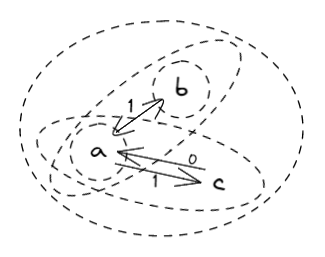
\includegraphics[width=0.3\textwidth]{Imagenes/grados_de_impacto.PNG}
  \caption{Grados de impacto para el espacio $X$ con la topología $\mathcal{A}$.}
  \label{fig:gradoImpacto}
\end{figure}

De la definición anterior se deduce el siguiente resultado:

\textbf{Teorema 3.1.3:} Los grados de impacto de una célula $x$ definen un sistema fundamental de vecindades.

\begin{proof}
Sea $x\in\mathcal{L}$ y $\mathcal{V}(x)$ una familia de vecindades de $x$. Defina el conjunto $A_0$ como el conjunto de puntos con grado de impacto con $x$ es igual a cero y de manera recursiva a los conjuntos $A_k$, cuyos elementos tienen grado de impacto con $x$ sea igual o menor a $k$. Claramente $A_i\subseteq A_j$ para $0\leq i\leq j$ y de ese modo $A_i\in\mathcal{V}(x)$ para $i=0,1,\cdots,n$.

Veamos ahora que el conjunto $A_0$ es la vecindad mínimal de $x$. Considere $y\in U_x$, en particular $y\in\bigcap\mathcal{V}(x)$ por la definición de 2.4.14. Si el grado de impacto de $y$ con $x$ es mayor a cero por la definición 3.1.2 podemos afirmar que existe $z\in\mathcal{L}$ tal que $z\thicksim x$, $z\thicksim y$ y $x\not\thicksim y$ y de ese modo $x$ e $y$ son puntos separables. Esto es una contradicción por el hecho de que $y\in \bigcap \mathcal{V}(x)$ y por lo tanto $y\thicksim_0 x$, es decir $y\in A_0$.

Considere $y\in A_0$ y por la definición de grado de impacto cero, afirmamos que los puntos $x$ e $y$ no son separables por lo que $y\in\mathcal{V}(x)$ y con esto concluimos la prueba.
\end{proof}

A continuación mostraremos algunas de las propiedades del conjunto $\mathcal{A}$ definido en la demostración anterior:

\textbf{Proposición 3.1.4:} Sea $x\in\mathcal{L}$ una célula y sea $\mathcal{A}$ la familia de conjuntos encajados definidos por el grado de impacto con $x$. Se cumplen las siguientes propiedades:

\begin{enumerate}
    \item El conjunto $\mathcal{A}$ posee elemento mínima igual a $A_0$,
    \item $\mathcal{A}$ es un conjunto ordenado finito con el orden de la contenencia, y
    \item $\mathcal{L}$ es un espacio uno-numerable.
\end{enumerate}

\begin{proof}
Cada numeral se deduce directamente de las definiciones 2.4.14, 2.4.16, 2.4.22 y el teorema 3.1.3.
\end{proof}

Algo que debemos tener en cuenta es que el grado de impacto por si solo no nos proporciona una medida del impacto que tienen los cambios de estado de células "lejanas" (o de grado de impacto mayor a cero). Estas medidas de impacto se entenderán como la probabilidad de que un cambio de estado afecte a la célula con la que estamos realizando la comparación, de ese modo las tasas de impacto serán valores entre 0 y 1.

\textbf{Ejemplo 3.1.5:} Las tasas de impacto pueden venir dadas por cualquier tipo de función en $[0,1]$, que tenga como dominio al conjunto de grados de impacto. 

Consideremos por ejemplo las siguientes matrices que describen los grados de impacto en tres distintos sistemas fundamentales de vecindades para la célula en la posición 2,2:

\begin{figure}[h]
  \centering
    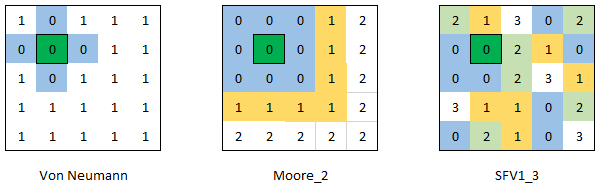
\includegraphics[width=0.7\textwidth]{Imagenes/ex315.PNG}
  \caption{Grados de impacto en diferentes sistemas de vecindades.}
  \label{fig:gradoImpacto}
\end{figure}

En la figura anterior podemos ver que debido a la manera en la que implementamos nuestro espacio de células, es posible representar los grados de impacto de cada una con una célula particular en un arreglo matricial, al igual que los estados de cada célula como se vio en el capítulo dos.

La asignación entre grados y tasas de impacto puede escogerse de cualquier manera dependiendo del contexto y la enfermedad que esté modelando. Para los efectos del ejemplo consideraremos las siguientes matrices de tasas de impacto:

\begin{figure}[h]
  \centering
    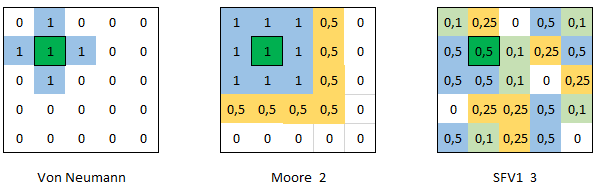
\includegraphics[width=0.7\textwidth]{Imagenes/ex3152.PNG}
  \caption{Tasas de impacto en diferentes sistemas de vecindades.}
  \label{fig:gradoImpacto}
\end{figure}

Una vez establecidos los conceptos de topología implementados para nuestro espacio $\mathcal{L}$ y sus sistemas fundamentales de vecindades podemos definir cada una de las reglas que implementaremos para cada modelo epidemiológico.

\section{Reglas de evolución}

En esta sección partiremos de una abstracción sobre la naturaleza de los modelos epidemiológicos definidos en el capítulo 2, esto nos permitirá definir de manera intuitiva las reglas de evolución de nuestros modelos en autómatas celulares.

Antes de comenzar a definir nuestras reglas de evolución definiremos las siguientes notaciones:
\begin{itemize}
    \item El estado de la célula $x$ en un momento $t$ se denotará como $\pi^t(x)$.
    \item La cantidad de individuos con grado de impacto $g$ y estado $K$ de una célula $x$ en un momento $t$ será representado como $\sigma_{g,K}^t(x)$.
    \item Para representar a la cantidad de individuos con un grado de impacto $g$ usaremos el símbolo $\Delta_g$. 
    \item Usaremos los símbolos $\mathcal{S}^t,\mathcal{I}^t,\mathcal{R}^t$ y $\mathcal{D}^t$ para denotar a los conjuntos de células susceptibles, infectadas, recuperadas y muertas respectivamente en el espacio $\mathcal{L}$ en el tiempo $t$. De manera formal
    $$\mathcal{S}^t=\{x\in\mathcal{L}:\pi^t(x)=S\},$$
    y de manera análoga se definen los conjuntos $\mathcal{I}^t,\mathcal{R}^t$ y $\mathcal{D}^t$. Note que $$\mathcal{S}^t\cup\mathcal{I}^t\cup\mathcal{R}^t\cup\mathcal{D}^t=\mathcal{L}\text{ para todo tiempo }t.$$
\end{itemize}

\subsection{Modelos SIS y SIR simples}

Recordemos que para las tasas de infección $\beta$ y de recuperación $\alpha$ los modelos SIS y SIR nos afirman que para $\mathcal{R}_0=\frac{\beta}{\alpha}>1$ la enfermedad será endémica. Trataremos de replicar inicialmente esté comportamiento de manera local sobre una célula analizando los siguientes puntos:

\begin{itemize}
    \item La probabilidad de que un individuo susceptible se enferme depende no solo de la enfermedad, sino que además depende de la cantidad de individuos infectados que tenga en su sistema de vecindades locales, atada a las tasas de impacto que definimos en la sección anterior. 
    \item Como vimos en el capítulo 1 la recuperación de los individuos infectados no se ve afectada por la cantidad de contactos con otras células y en lugar de eso depende completamente de la tasa de recuperación $\alpha$, la cual en nuestro caso entenderemos como la proporción de individuos infectados que se recuperan de la enfermedad.
    \item Para el estado de inmunidad en el modelo SIR, supondremos que los individuos que posean este estado se mantendrán inmunes. Esto quiere decir que la transformación para individuos recuperados será constante.
\end{itemize}

Dado que los modelos SIS y SIR comparten el paso del estado S al estado I definiremos primero la regla de evolución para un modelo SI:

\textbf{Definición 3.2.1:} Para una célula $x$ en un espacio $\mathcal{L}$ definimos la regla SI como:
\begin{equation}
    \phi_{SI}^t(x)=\left\{\begin{array}{ll}
        S & \text{si }\pi^t(x)=S\text{, }\sum_g{\sigma_{g,I}^t(x)\cdot P(g)}\leq \sum_g{\sigma_{g,S}^t(x)\cdot P(g)}\text{ y }\rho\geq i(t),\\
        I & \text{en otro caso,}
    \end{array}\right.
\end{equation}
con $\rho\in\mathcal{U}_{[0,1]}$, $P(g)$ la tasa de impacto del grado $g$ e
\begin{equation}
    i(t) = \frac{\beta}{\alpha}\sum_g{\frac{\sigma_{g,I}^t(x)}{\Delta_g}}\cdot P(g).
\end{equation}

\textbf{Ejemplo:} En la figura imagen podemos encontrar la configuración de estados para un sistema de 25 células y en las últimas tres, encontramos la disposición de grados de impacto para las tres células marcadas en color verde (primera imagen).
\begin{figure}[h]
  \centering
    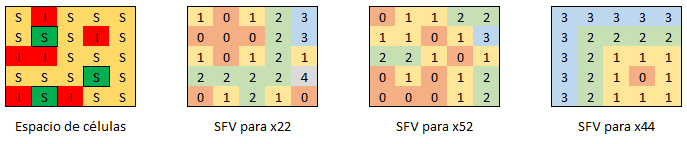
\includegraphics[width=0.9\textwidth]{Imagenes/cellSpace.PNG}
\end{figure}\\
Donde SFV es una abreviación de Sistema Fundamental de Vecindades.\\
Para este ejemplo consideraremos las siguientes tasas de impacto:\\

\begin{table}[h]
\begin{center}
\begin{tabular}{| c | c |}
\hline
\multicolumn{2}{ |c| }{Relación grado/tasa} \\ \hline
Grados & Tasas \\ \hline
0 & 0.5 \\
1 & 0.3\\
2 & 0.25\\
3 & 0.1\\ 
4 & 0.05\\ \hline
\end{tabular}
\caption{Relación entre tasas y grados de impacto.}
\end{center}
\end{table}
A continuación calcularemos las magnitudes ponderadas de individuos susceptibles e infectados y la probabilidad de infectarse para cada una de las tres células:

\begin{itemize}
    \item Célula $x_{2,2}$:
    \begin{align*}
    \begin{array}{l}
        \sum_g\sigma_{g,S}^0(x_{2,2})\cdot P(g) = 4\cdot0.5+6\cdot0.3+6\cdot0.25+2\cdot0.1+1\cdot0.05 = 5.55 \\
        \sum_g\sigma_{g,I}^0(x_{2,2})\cdot P(g) = 3\cdot0.5+1\cdot0.3+2\cdot0.25+0\cdot0.1+0\cdot0.05 = 2.3\\
        i_{2,2}(0) = \frac{\beta}{\alpha}\cdot\left(\frac{3\cdot0.5}{7}+\frac{1\cdot0.3}{7}+\frac{2\cdot0.25}{8}+\frac{0\cdot0.1}{2}+\frac{0\cdot0.05}{1}\right)=\frac{179}{560}\cdot\frac{\beta}{\alpha}
    \end{array}
    \end{align*}
    \item Célula $x_{5,2}$:
    \begin{align*}
    \begin{array}{l}
        \sum_g\sigma_{g,S}^0(x_{5,2})\cdot P(g) = 6\cdot0.5+8\cdot0.3+4\cdot0.25+1\cdot0.1+0\cdot0.05 = 6.5 \\
        \sum_g\sigma_{g,I}^0(x_{5,2})\cdot P(g) = 2\cdot0.5+2\cdot0.3+2\cdot0.25+0\cdot0.1+0\cdot0.05 = 2.1\\
        i_{5,2}(0) = \frac{\beta}{\alpha}\cdot\left(\frac{2\cdot0.5}{8}+\frac{2\cdot0.3}{10}+\frac{2\cdot0.25}{6}+\frac{0\cdot0.1}{1}\right)=\frac{161}{600}\cdot\frac{\beta}{\alpha}
    \end{array}
    \end{align*}
    \item Célula $x_{4,4}$:
    \begin{align*}
    \begin{array}{l}
        \sum_g\sigma_{g,S}^0(x_{4,4})\cdot P(g) = 1\cdot0.5+7\cdot0.3+5\cdot0.25+6\cdot0.1+0\cdot0.05 = 4.45 \\
        \sum_g\sigma_{g,I}^0(x_{4,4})\cdot P(g) = 0\cdot0.5+1\cdot0.3+2\cdot0.25+3\cdot0.1+0\cdot0.05 = 1.1\\
        i_{4,4}(0) = \frac{\beta}{\alpha}\cdot\left(\frac{0\cdot0.5}{1}+\frac{1\cdot0.3}{8}+\frac{2\cdot0.25}{7}+\frac{3\cdot0.1}{9}\right)=\frac{239}{1680}\cdot\frac{\beta}{\alpha}
    \end{array}
    \end{align*}
\end{itemize}
En este caso las tres células pueden o no contagiarse de la enfermedad si aplicamos la regla $\phi_{SI}^t(x)$. Supongamos que la enfermedad cuenta con una tasa de infección $\beta=0.5$ y una tasa $\alpha=0.2$, de ese modo las probabilidades de adquirir la enfermedad son:
$$\begin{array}{ccccc}
    i_{2,2}(0)=0.8, & i_{5,2}(0)=0.675. & \text{e} & i_{4,4}(0)=0.35.
\end{array}$$
Podemos observar que la célula $x_{4,4}$ tiene una probabilidad menor de adquirir la enfermedad, esto se debe a que según el sistema de vecindades escogido la célula se encuentra más alejada de los infectados que las células $x_{2,2}$ y $x_{5,2}$.\\

La definición 3.2.1 nos permite definir de manera natural a las reglas de evolución para los modelos SIS y SIR en autómatas celulares:

\textbf{Definición 3.2.2:} Dada una célula $x$ en un conjunto $\mathcal{L}$ definimos respectivamente las reglas de evolución para los modelos SIS y SIR respectivamente como:
\begin{equation}
    \phi_{SIS}^t(x)=\left\{\begin{array}{ll}
        \phi_{SI}^t(x) & \text{si }\pi^t(x) = S,\\
        I & \text{si }\pi^t(x)=I\text{ y }\rho>\alpha,\\
        S & \text{si }\pi^t(x)=I\text{ y }\rho\leq\alpha.
    \end{array}\right.
\end{equation}

\begin{equation}
    \phi_{SIR}^t(x)=\left\{\begin{array}{ll}
        \phi_{SI}^t(x) & \text{si }\pi^t(x) = S,\\
        I & \text{si }\pi^t(x)=I\text{ y }\rho>\alpha,\\
        R & \text{si }\pi^t(x)=I\text{ y }\rho\leq\alpha, y \\
        R & \text{si }\pi^t(x)=R,
    \end{array}\right.
\end{equation}
donde $\rho\in\mathcal{U}_{[0,1]}$.

\textbf{Ejemplo:}
\subsection{Modelos con natalidad y mortalidad}
Partiendo del principio de que los análisis desarrollados en nuestra investigación tengan una mayor aplicabilidad en el ámbito epidemiológico decidimos separarnos un poco de los modelos clásicos, ya que en estos se supone que las tasas de natalidad y mortalidad son iguales y esto no necesariamente se cumple en el mundo real.

La segunda característica que tendremos en mente para definir nuestra regla de evolución parte de hipótesis de que los individuos en un sistema tienen una probabilidad de fallecer por causas ajenas a la enfermedad que depende de la edad del mismo individuo.

Para implementar la noción de edad de una célula inicialmente tendremos que modificar el dominio de nuestra regla de evolución. Para estos modelos debemos tener en cuenta el estado de la célula central junto con su edad y el estado de sus vecinos, de modo que 
$$Dom(\phi_\mu)=\Sigma_x\times K\times\overbrace{\Sigma\times\cdots\times\Sigma}^N\text{, con }K=\{1,2,\cdots,100\},$$
si suponemos que la edad de la célula $x$ puede ir de 1 a 100 unidades temporales (semanas, meses, años, etc.).

Otra característica que podemos implementar en nuestro modelo es la del envejecimiento de las células, esto con el objetivo de analizar el impacto de una enfermedad sobre los individuos de un sistema en diferentes etapas de su "vida". La manera en la que abordaremos esta idea será con el siguiente ajuste en el rango de nuestra regla
$$Ran(\phi_\mu)=\Sigma_x\times K.$$
Dado que estamos trabajando sobre poblaciones de tamaño constante la manera en la que interpretaremos el nacimiento de una célula será con la ocupación del espacio que deja una que muere. Para esto identificaremos a los espacios que dejan las células que mueren con el estado $D$ y una edad cero, esto nos permitirá separar a los espacios que pueden ocuparse y los que no de células que interactúen con sus vecinos. Al igual que en los modelos descritos en el capítulo 1 asumiremos que los individuos que "nacen" son susceptibles a la enfermedad.

Teniendo estas ideas en mente podemos definir la regla de evolución para un modelo epidemiológico $M$ de la siguiente manera:

\textbf{Definición 3.2.3:} Sea $x$ una célula en un conjunto $\mathcal{L}$, $M$ un modelo epidemiológico y $T$ una unidad temporal (días, meses, años, etc.). Definimos la regla de evolución con nacimientos y muertes para $M$ como:
\begin{equation}
    \mu_{M,T}^t(x)=\left\{\begin{array}{ll}
        D,0 & \text{si }t\not\equiv 0 \text{ (modulo }T\text{), }\pi^t(x)\in\{S,I,R\}\text{ y }\rho\leq\omega_k, \\
        D,0 & \text{si }\pi^t(x)=D\text{ y }\rho>b,\\
        S,1 & \text{si }\pi^t(x)=D\text{ y }\rho\leq b,\\
        \phi_M^t(x),E^t(x) & \text{si }t\not\equiv 0 \text{ (modulo }T),\\
        \phi_M^t(x),E^t(x)+1 & \text{si }t\equiv 0 \text{ (modulo }T),
    \end{array}\right.
\end{equation}
donde $\omega_k$ es la probabilidad de morir por causas ajenas a la enfermedad para las edades en la partición k-ésima del intervalo $[0,100]$, $b$ es la tasa de natalidad, $\phi_M^t$ es la regla de evolución del modelo epidemiológico, $E^t(x)$ denota la edad de la célula $x$ en el momento $t$ y $\rho\in\mathcal{U}_{[0,1]}$.
\subsection{Modelos con muerte por enfermedad}
En esta sección nos enfocaremos en definir la versión más general de los modelos epidemiológicos clásicos en ecuaciones diferenciales definidas en el capítulo 1. La muerte por enfermedad afectará únicamente a las células que posean la enfermedad y, buscando una mayor aplicabilidad sobre eventos más realistas asumiremos que la enfermedad puede tener un mayor impacto mortal sobre algunas edades. 

Al igual que en la sección anterior, realizaremos una partición sobre el intervalo $[0,100]$ y definiremos una probabilidad $\theta_k$ que indique la probabilidad de morir a causa de la enfermedad en la k-ésima partición. De manera formal:

\textbf{Definición 3.2.4:} Sea $x$ una célula en un conjunto $\mathcal{L}$, $M$ un modelo epidemiológico y $T$ una unidad temporal (días, meses, años, etc.). Definimos la regla de evolución con muerte por enfermedad para $M$ como:
\begin{equation}
    \theta_{M,T}^t(x)=\left\{\begin{array}{ll}
        D,0 & \text{si }\pi^t(x)=I\text{ y }\rho\leq\theta_k, \\
        \mu_{M,T}^t(x) & \text{en otro caso.}
    \end{array}\right.
\end{equation}
Donde $\theta_k$ es la probabilidad de morir por la enfermedad para los individuos con una edad en el intervalo k-ésimo de la partición del intervalo $[0,100]$, $\mu_{M,T}^t$ es la regla de evolución para modelos con nacimientos y muertes y $\rho\in\mathcal{U}_{[0,1]}$.

En el siguiente capítulo profundizaremos sobre la manera en la que una enfermedad con unas características dadas, se comporta en un conjunto de células tanto en los modelos clásicos como en autómatas celulares. Esto nos permitirá validar cada una de las reglas definidas en el presente capítulo y nos brindará un punto de vista espacial sobre las dinámicas de una enfermedad.